\chapter{Realni brojevi}\label{ch:realni-brojevi}

\section{Računanje s realnim brojevima}\label{sec:računanje-s-realnim-brojevima}

Skup je bilo koja kolekcija različitih objekata u cjelini.

Elementi skupa mogu biti raznih vrsta: brojevi, ljudi, slova abecede, drugi skupovi itd.
Skupovi se dogovorno označavaju velikim slovima $A$, $B$, $C$, $\ldots$ te vitičastim zagradama $\{\ \}$ u koje se upisuju elementi.
Skupovi se mogu definirati, tj.\ opisati riječima ili eksplicitnim nabrajanjem svih elemenata između vitičastih zagrada.
Skup može biti konačan, beskonačan ili prazan.

Ako je nešto element nekog pojedinačnog skupa, odnosno pripada skupu, tada koristimo oznaku $\in$, a u slučaju da nije element skupa odnosno ne pripada skupu oznaku $\notin$.

Skupove možemo uspoređivati, pa ukoliko su svi elementi skupa $A$ i $B$ isti, možemo reći da je skup $A$ jednak skupu $B$, a tvrdnju zapisujemo $A = B$.
Nisu li svi elementi skupa $A$ i $B$ isti možemo zaključiti da je skup $A$ različit od skupa $B$, a tvrdnju zapisujemo $A \neq B$.

Ako je svaki član skupa $A$ također član skupa $B$, tada se za skup $A$ kaže da je podskup skupa $B$, a zapisuje se $A \subseteq B$.
Može se, također, zapisati $B \supseteq A$ odnosno skup $B$ je nadskup skupa $A$.
Ako je skup $A$ podskup i nije jednak skupu $B$, tada se za skup $A$ kaže da je pravi podskup skupa $B$, a zapisuje se $A \subset B$ ili možemo reći da je skup $B$ pravi nadskup skupa $A$ i zapisati $B \supset A$ kako prikazuje slika~\ref{fig:podskup}.

\begin{figure}
\begin{center}\vspace{0.25cm}
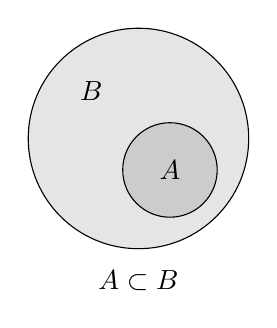
\begin{tikzpicture}[scale=0.8, every node/.style={scale=1}]
\filldraw[fill=gray!20,draw=black] (0,0) circle [radius=1.75];
\filldraw[fill=gray!40,draw=black] (0.5,-0.5) circle [radius=0.75];
\node at (0.5,-0.5) {$A$};
\node at (-0.75,0.75) {$B$};
\node at (0,-2.25) {$A \subset B$};
\end{tikzpicture}
\end{center}
\caption{Podskup}\label{fig:podskup}
\end{figure}

Postoji nekoliko načina za konstruiranje novih skupova od već postojećih.
Dva se skupa mogu \emph{zbrojiti} i to nazivamo unija skupova.
Unija skupova $A$ i $B$, označena sa $A \cup B$, je skup svih elemenata koji su članovi ili skupa $A$ ili skupa $B$.

Novi se skup također može konstruirati određivanjem \emph{zajedničkih} elemenata obaju skupova.
To nazivamo presjek skupova.
Presjek skupova $A$ i $B$, označen sa $A \cap B$, je skup svih elemenata koji su članovi i skupa $A$ i skupa $B$.
Slika~\ref{fig:operacije-sa-skupovima} prikazuje uniju i presjek skupova pomoću Vennovih dijagrama.

\begin{figure}[h!]
\begin{center}\vspace{0.25cm}
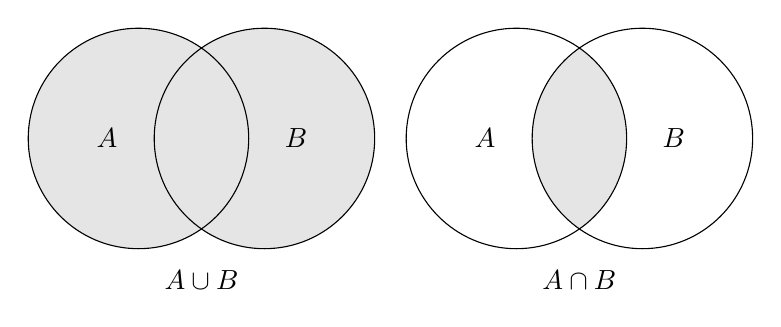
\begin{tikzpicture}[scale=0.8, every node/.style={scale=1}]
\filldraw[fill=gray!20,draw=black] (4,0) circle [radius=1.75] (6,0) circle [radius=1.75];
\node at (3.5,0) {$A$};
\node at (6.5,0) {$B$};
\node at (5,-2.25) {$A \cup B$};
\begin{scope}
  \clip (10,0) circle [radius=1.75];
  \fill[fill=gray!20] (12,0) circle [radius=1.75];
\end{scope}
\draw (10,0) circle [radius=1.75] (12,0) circle [radius=1.75];
\node at (9.5,0) {$A$};
\node at (12.5,0) {$B$};
\node at (11,-2.25) {$A \cap B$};
\end{tikzpicture}
\end{center}
\caption{Operacije sa skupovima}\label{fig:operacije-sa-skupovima}
\end{figure}

\subsection{Skup prirodnih brojeva}\label{subsec:skup-prirodnih-brojeva}
Skup prirodnih brojeva označavamo s oznakom $\mathbb{N}$.
Ovaj skup je zatvoren s obzirom na zbrajanje i množenje.
\[ \mathbb{N}=\{1,2,3,4,5,\ldots\}. \]
Skup se često proširuje brojem 0 te ga u tom slučaju označavamo s $\mathbb{N}_0$.
Kažemo da je prirodni broj $n$ djeljiv s prirodnim brojem $m$ ako postoji $k \in \mathbb{N}$ sa svojstvom da je $n=k \cdot m$.
Tada je $n$ višekratnik broja $m$ te je $m$ djelitelj broja $n$ ili kraće $m|n$.

U skupu prirodnih brojeva svaki broj ima svog neposrednog sljedbenika ($n+1$), a samim time, osim broja 1, i svog neposrednog prethodnika ($n-1$).

Najveći zajednički djelitelj prirodnih brojeva $a$, $b$ i $c$ je najveći broj koji dijeli sve te brojeve i označavamo ga nzd ($a$, $b$, $c$), a najmanji zajednički višekratnik prirodnih brojeva $a$, $b$ i $c$ je najmanji prirodni broj koji je djeljiv sa svakim od tih brojeva i označavamo ga nzv ($a$, $b$ i $c$).

Prirodan broj veći od 1 je prost broj ako je djeljiv samo s 1 i sa samim sobom.
Broj je složen ako nije prost, s iznimkom broja 1 koji ne držimo ni prostim ni složenim.
Svaki se prirodan broj može napisati u obliku umnoška prostih brojeva.